\FloatBarrier


\begin{figure}[htbp]
	\begin{minipage}[b]{0.5\textwidth} 
		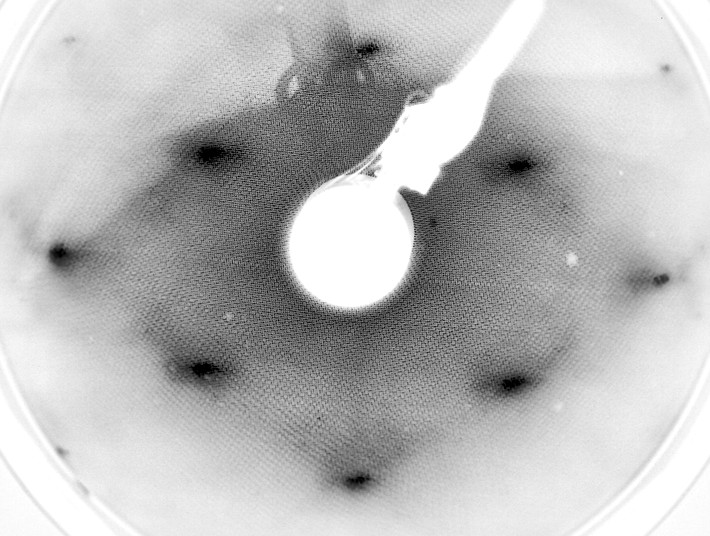
\includegraphics[width=\textwidth]{LEED-Bilder/bearbeitet/unbedampft_E207}
		\label{Bild} 
	\end{minipage}
	\hfill
	\begin{minipage}[b]{0.5\textwidth}
		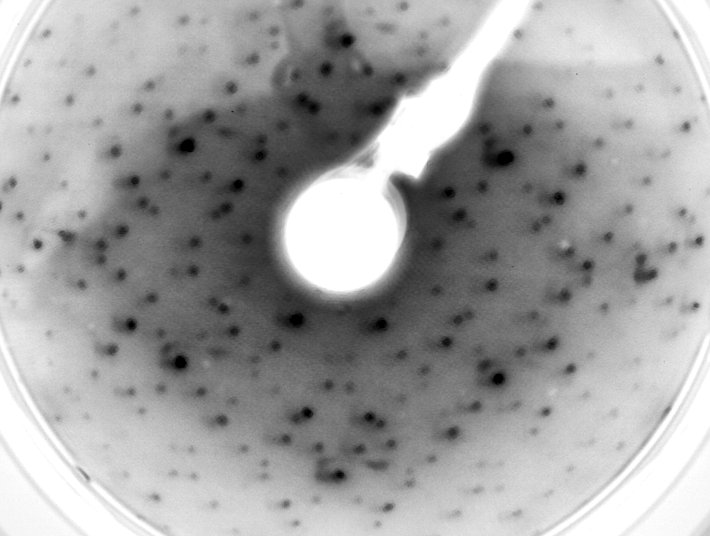
\includegraphics[width=\textwidth]{LEED-Bilder/bearbeitet/unbedampft_E207_MitteKristall.jpg}
		\label{Bild} 
	\end{minipage}
	\caption{\textit{Links der Re-Kristall mit scharfen Spots und eindeutiger Struktur. Rechts die
	Re-Oberfläche mit Verschmutzung, zu erkennen an der Überstruktur und den schwächeren Hauptspots.}}
\end{figure}

\begin{figure}[htbp]
		\captionsetup{name=Abb.}
	\begin{minipage}[b]{0.5\textwidth} 
		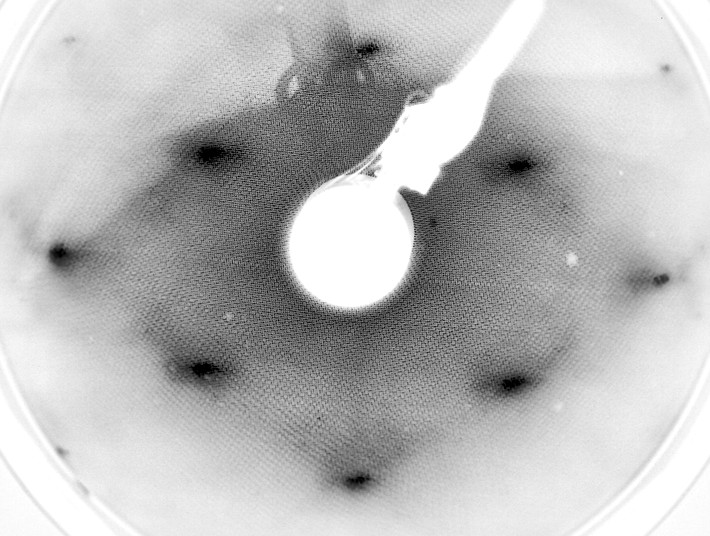
\includegraphics[width=\textwidth]{LEED-Bilder/bearbeitet/unbedampft_E207}
		\caption{\textit{Re-Oberfläche}}
		\label{Bild} 
	\end{minipage}
	\hfill
	\begin{minipage}[b]{0.5\textwidth}
		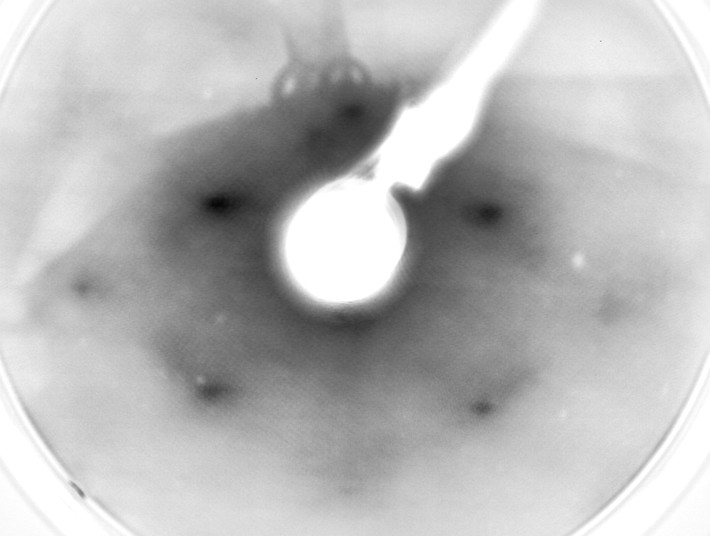
\includegraphics[width=\textwidth]{LEED-Bilder/bearbeitet/0_5ML_E208}
		\caption{\textit{1/2 Monolage Au}}
		\label{Bild} 
	\end{minipage}
	
	\begin{minipage}[b]{0.5\textwidth} 
		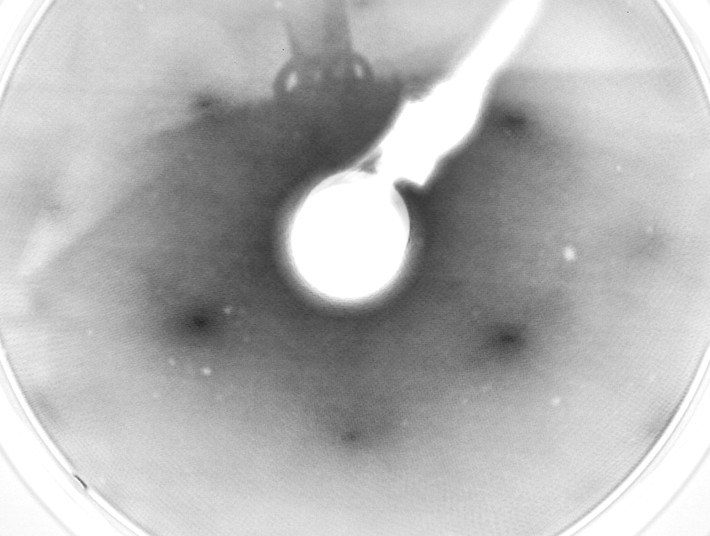
\includegraphics[width=\textwidth]{LEED-Bilder/bearbeitet/1ML_E207}
		\caption{\textit{1 Monolage Au}}
		\label{Bild} 
	\end{minipage}
	\hfill
	\begin{minipage}[b]{0.5\textwidth}
		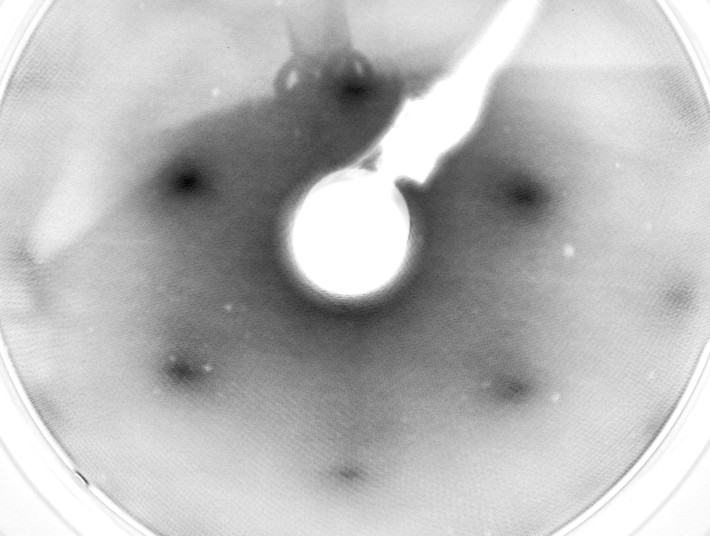
\includegraphics[width=\textwidth]{LEED-Bilder/bearbeitet/6ML_E207}
		\caption{\textit{6 Monolagen Au}}
		\label{Bild} 
	\end{minipage}
	
	\begin{minipage}[b]{0.5\textwidth} 
		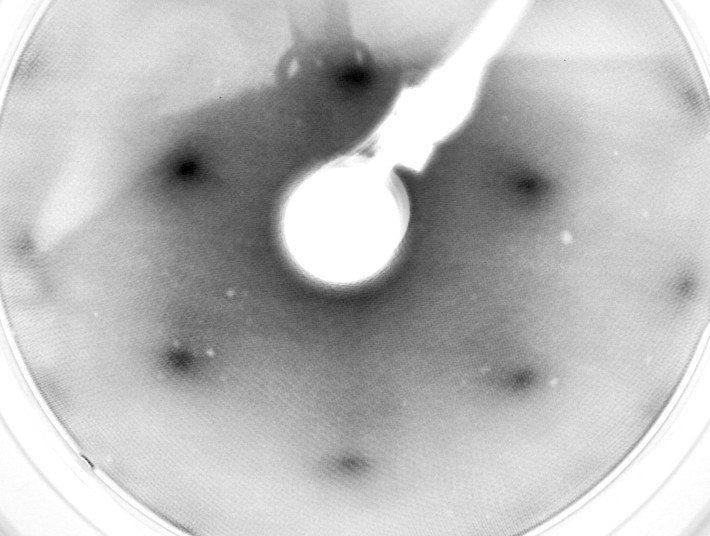
\includegraphics[width=\textwidth]{LEED-Bilder/bearbeitet/10ML_E207}
		\caption{\textit{10 Monolagen Au}}
		\label{Bild} 
	\end{minipage}
	\hfill
	\begin{minipage}[b]{0.5\textwidth}
		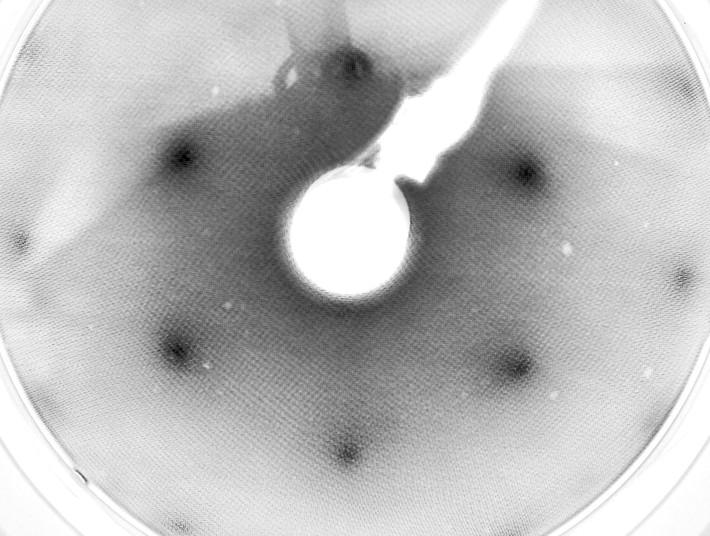
\includegraphics[width=\textwidth]{LEED-Bilder/bearbeitet/30ML_E208}
		\caption{\textit{30 Monolagen Au}}
		\label{Bild} 
	\end{minipage}
	\caption{noch eine Caption}
\end{figure}


\FloatBarrier